\section{Tổng quan kiến trúc hệ thống}
\subsection{Yêu cầu thiết kế hệ thống}

Hệ thống GraphRAG được thiết kế dựa trên năm yêu cầu rút từ bài toán hỏi-đáp về nghệ thuật Chèo, chia thành hai nhóm: \textit{yêu cầu chức năng} (tập trung vào chất lượng kết quả mà hệ thống phải tạo ra), và \textit{yêu cầu phi chức năng} (tập trung vào cách hệ thống được tổ chức và vận hành). Mỗi yêu cầu sẽ được giải quyết ở các mục thiết kế tiếp theo và được kiểm chứng ở Chương~4.

\textbf{Yêu cầu chức năng} gồm ba yêu cầu chính về chất lượng câu trả lời:

\begin{itemize}
  \item \textbf{Thống nhất với tri thức nguồn.} Câu trả lời chỉ được dùng các thực thể, quan hệ và sự kiện có trong đồ thị tri thức Chèo, không được bịa nhân vật, vở diễn hay diễn viên không có trong cơ sở dữ liệu nguồn. Đây là yêu cầu quan trọng nhất với một miền văn hoá truyền thống, vì sai về tên riêng hay quan hệ giữa các thực thể có thể gây hiểu sai về di sản.

  \item \textbf{Khả năng bao phủ đa mức độ truy vấn.} Hệ thống cần trả lời được cả ba mức câu hỏi: tra cứu trực tiếp một thực thể (\textit{Local}, ví dụ ``Ai đóng vai Thị Màu?''), tổng hợp trong một cụm thực thể có liên kết chặt (\textit{Community}, ví dụ ``Diễn viên nào đóng cả hai vở Quan Âm Thị Kính và Kim Nham?''), và so sánh xuyên nhiều vở (\textit{Global}, ví dụ ``So sánh số phận của Súy Vân và Thị Kính''). Một hệ thống chỉ tốt ở một mức sẽ không đáp ứng được nhu cầu thực tế của người dùng.

  \item \textbf{Đảm bảo chất lượng câu trả lời.} Câu trả lời phải đầy đủ thông tin được hỏi, dễ đọc, trả lời bằng tiếng Việt một cách tự nhiên và phù hợp với cách dùng từ trong nghệ thuật Chèo. Đây là điều kiện để hệ thống thực sự hữu ích với người dùng phổ thông, bên cạnh việc sử dụng đúng tri thức.
\end{itemize}

\textbf{Yêu cầu phi chức năng} gồm hai yêu cầu chính về kiến trúc và vận hành:

\begin{itemize}
  \item \textbf{Không phụ thuộc cứng vào mô hình ngôn ngữ.} Các mô hình ngôn ngữ phát triển nhanh, vì vậy kiến trúc phải cho phép thay LLM - đổi nhà cung cấp, đổi phiên bản hay chuyển sang chạy nội bộ - qua cấu hình mà không phải sửa logic truy xuất hay tri thức miền. Yêu cầu này giúp hệ thống không bị ràng buộc vào một mô hình duy nhất và có thể tận dụng các mô hình mới khi xuất hiện.

  \item \textbf{Có khả năng triển khai và mở rộng trong thực tế.} Hệ thống phải chạy được trên hạ tầng đám mây phục vụ nhiều người dùng cùng lúc, và cho phép cập nhật, mở rộng tri thức - thêm vở mới hay bổ sung quan hệ - mà không phải tái thiết kế các thành phần khác. Đây là điều kiện để hệ thống không hoàn toàn chỉ hiệu quả về mặt lý thuyết và còn có giá trị thực nghiệm.
\end{itemize}

\subsection{Kiến trúc phân tầng của hệ thống}

Hệ thống GraphRAG được thiết kế theo kiến trúc phân tầng (Hình~\ref{fig:4-layer}), với mục tiêu tách biệt rõ ràng vai trò của từng thành phần để hỗ trợ mở rộng và bảo trì. Hệ thống gồm bốn tầng: (i) tầng giao diện người dùng, (ii) tầng xử lý GraphRAG, (iii) tầng tri thức, và (iv) tầng mô hình ngôn ngữ. Cách phân chia này cho phép thay thế hoặc nâng cấp một tầng hay thay đổi cơ sở tri thức mà không ảnh hưởng đến logic của các tầng còn lại.

\begin{figure}[ht!]
    \centering
    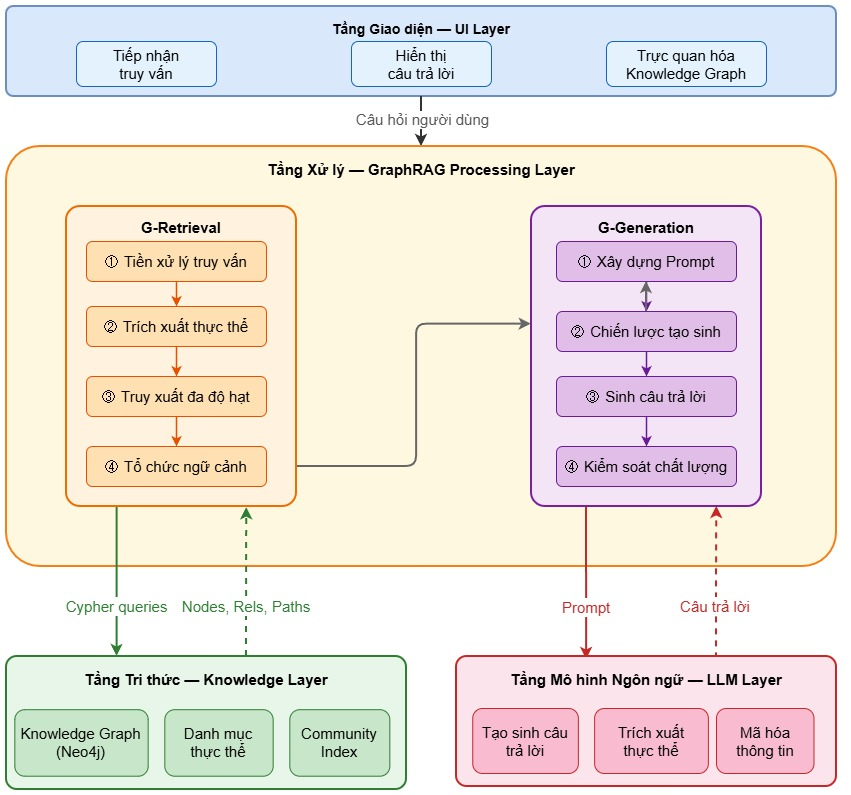
\includegraphics[width=0.9\linewidth]{figures//c3/4-layer.jpg}
    \caption{Thiết kế 4 tầng của hệ thống GraphRAG}
    \label{fig:4-layer}
\end{figure}

\textbf{Tầng giao diện người dùng} đóng vai trò là cầu nối tương tác giữa người dùng và hệ thống. Tầng này tiếp nhận câu hỏi ngôn ngữ tự nhiên từ phía người dùng và hiển thị câu trả lời do hệ thống sinh ra. Ngoài ra, tầng giao diện còn cung cấp môi trường trực quan để trình bày các thông tin phụ trợ như tập thực thể liên quan hay đường truy xuất, qua đó hỗ trợ người dùng kiểm chứng nguồn gốc câu trả lời.

\textbf{Tầng xử lý GraphRAG} đóng vai trò trung tâm, điều phối toàn bộ luồng xử lý từ khi nhận câu hỏi đến khi sinh ra câu trả lời. Tầng này được tổ chức thành hai phân hệ chính: \textbf{G-Retrieval} chịu trách nhiệm trích xuất tri thức phù hợp từ đồ thị tri thức, và \textbf{G-Generation} chịu trách nhiệm tổng hợp ngữ cảnh đó thành câu trả lời thông qua mô hình ngôn ngữ.

\textbf{Tầng tri thức} là nơi lưu trữ và quản lý toàn bộ tri thức miền nghệ thuật Chèo dưới dạng đồ thị tri thức. Bên cạnh chức năng lưu trữ, tầng này còn duy trì các cơ chế lập chỉ mục đa mức và bộ quy tắc suy luận quan hệ. Việc này giúp tăng tốc truy xuất và mở rộng phạm vi các tri thức ngầm tồn tại trong đồ thị tri thức. Nhờ cấu trúc đồ thị, hệ thống có thể mở rộng ngữ cảnh thông qua các quan hệ giữa thực thể và hỗ trợ hiệu quả những câu hỏi yêu cầu suy luận đa bước.

\textbf{Tầng mô hình ngôn ngữ} cung cấp năng lực sinh ngôn ngữ thông qua việc gọi các API LLM. Tầng xử lý GraphRAG sử dụng tầng này ở hai thời điểm: phân tích và trích xuất thực thể từ câu hỏi trong G-Retrieval, và tạo sinh câu trả lời dựa trên ngữ cảnh đã chuẩn bị trong G-Generation. Cách tổ chức tách rời này cho phép thay thế mô hình ngôn ngữ mà không ảnh hưởng đến các tầng còn lại, đồng thời duy trì ranh giới rõ ràng giữa logic nghiệp vụ và năng lực mô hình.

Trọng tâm của khoá luận tập trung vào tầng tri thức và tầng xử lý GraphRAG - hai tầng quyết định chất lượng tri thức và hành vi truy xuất của hệ thống. Hai tầng còn lại đóng vai trò hỗ trợ: tầng giao diện cung cấp tương tác với người dùng, còn tầng mô hình ngôn ngữ được triển khai để tận dụng các mô hình trí tuệ nhân tạo mãnh mẽ hiện nay. Các mục tiếp theo của chương lần lượt trình bày chi tiết hai tầng cốt lõi cùng các cơ chế vận hành đi kèm.

\subsection{Luồng xử lý tổng thể}

Mỗi câu hỏi của người dùng sẽ thông qua tầng giao diện để xuống tới tầng xử lý GraphRAG, trải qua hai phân hệ xử lý trước khi hệ thống trả câu trả lời ở dạng ngôn ngữ tự nhiên cho người dùng(Hình~\ref{fig:overview}).Phân hệ thứ nhất là \textbf{G-Retrieval}, có trách nhiệm tiếp nhận câu hỏi ngôn ngữ tự nhiên và xây dựng lên ngữ cảnh từ đồ thị tri thức. Phân hệ thứ hai là \textbf{G-Generation}, có nhiệm vụ tổng hợp ngữ cảnh đó thành câu trả lời thông qua mô hình ngôn ngữ.

\begin{figure}[ht!]
    \centering
    \includegraphics[width=0.9\linewidth]{figures/c3/graphrag_overview.jpg}
    \caption{Tổng quan luồng xử lý của hệ thống GraphRAG.}
    \label{fig:overview}
\end{figure}

Phân hệ G-Retrieval thực hiện ba giai đoạn tuần tự. \textit{Giai đoạn 1 - Tiền xử lý và trích xuất thực thể}: câu hỏi gốc được mô hình ngôn ngữ mở rộng và phân rã thành tập truy vấn đã được làm giàu, đồng thời trích xuất tập thực thể liên quan (được đối chiếu với Danh mục thực thể nhằm đảm bảo mọi thực thể đầu ra đều tồn tại trong đồ thị tri thức). \textit{Giai đoạn 2 - Truy vấn đa mức độ}: dựa trên tập thực thể đã trích xuất, hệ thống thực hiện truy xuất trên đồ thị tri thức theo bốn mức độ Node, Triplet, Path và Subgraph; kết quả được tổng hợp thành đối tượng dữ liệu đồ thị chứa tri thức ở các phạm vi từ thực thể đơn lẻ đến cụm các thực thể có mối liên hệ với nhau. \textit{Giai đoạn 3 - Tổ chức ngữ cảnh}: dữ liệu đồ thị được chuyển đổi sang bốn định dạng văn bản - mô tả tự nhiên, bảng kề, JSON và chuỗi nút - phù hợp với mô hình ngôn ngữ. Đồng thời, cũng từ các dữ liệu đồ thị này, hệ thống trích xuất ra tập các dữ kiện chính - tóm lược các thông tin cốt lõi cần thiết cho câu trả lời. Đầu ra của G-Retrieval là tập ngữ cảnh đa định dạng kèm tập dữ kiện chính tương ứng.

Phân hệ G-Generation nhận tập ngữ cảnh, tập dữ kiện chính và câu hỏi gốc, sau đó xây dựng câu trả lời theo hai giai đoạn. \textit{Giai đoạn 1 - Xây dựng prompt}: bốn thành phần gồm tiêu đề ngữ cảnh, tập dữ kiện chính, khối ngữ cảnh đa định dạng và câu hỏi kèm chỉ dẫn được tổ hợp thành prompt hoàn chỉnh. \textit{Giai đoạn 2 - Chiến lược tạo sinh}: prompt được gửi tới mô hình ngôn ngữ theo một trong ba chiến lược Pre, Mid hoặc Post, khác nhau ở mức độ kiểm soát quá trình suy luận và số lượt gọi mô hình. Câu trả lời được trả về tầng giao diện và hiển thị cho người dùng.

Toàn bộ quy trình tách biệt rõ ràng giữa truy xuất tri thức và sinh ngôn ngữ: tri thức được xác định, lọc và đóng gói trong G-Retrieval; mô hình ngôn ngữ chỉ tham gia với vai trò sinh ngôn ngữ dựa trên ngữ cảnh đã được chuẩn bị. Bên cạnh đồ thị tri thức được truy vấn tại thời điểm thực thi, hệ thống duy trì Danh mục thực thể - bản trích xuất tên thực thể được nạp từ đồ thị tại thời điểm khởi tạo hệ thống - đóng vai trò là ràng buộc cho giai đoạn trích xuất thực thể của G-Retrieval.